% !TeX program = lualatex
% !TeX encoding = utf8
% !TeX spellcheck = uk_UA
% !TeX root =../LabWork.tex

%------------- Externalize ------------
%\usetikzlibrary{external}
%\tikzexternalize[prefix=\currfiledir/pictures/]
%\tcbsetforeverylayer{shield externalize}


%============================================= Заголовок документу ====================================================%

\keywords{Змінний струм, $RC$-коло, активний опір, ємнісний опір,імпеданс.}
\abstract{Визначення імпедансу конденсатора як функції частоти. Визначення фазового зсуву між напругою на конденсаторі та струмом в колі як функції частоти.}
\apparatus{генератор сигналів низькочастотний ГЗ-112, диференційний підсилювач, осцилограф C1-93.}
\chapter{Конденсатор у колі змінного струму}
\makeworktitle

%======================================================================================================================%



\section{Обладнання}

\subsubsection*{Генератор ГЗ-112}

\begin{figure}[h!]
\centering
\begin{tikzpicture}[every pin/.style={minimum size = 5pt, pin edge={red, thick}, draw, fill=gray!5, red, circle, font=\scriptsize},
    small dot/.style={fill=black,circle,scale=0.3}]
    \node at (0,0){ 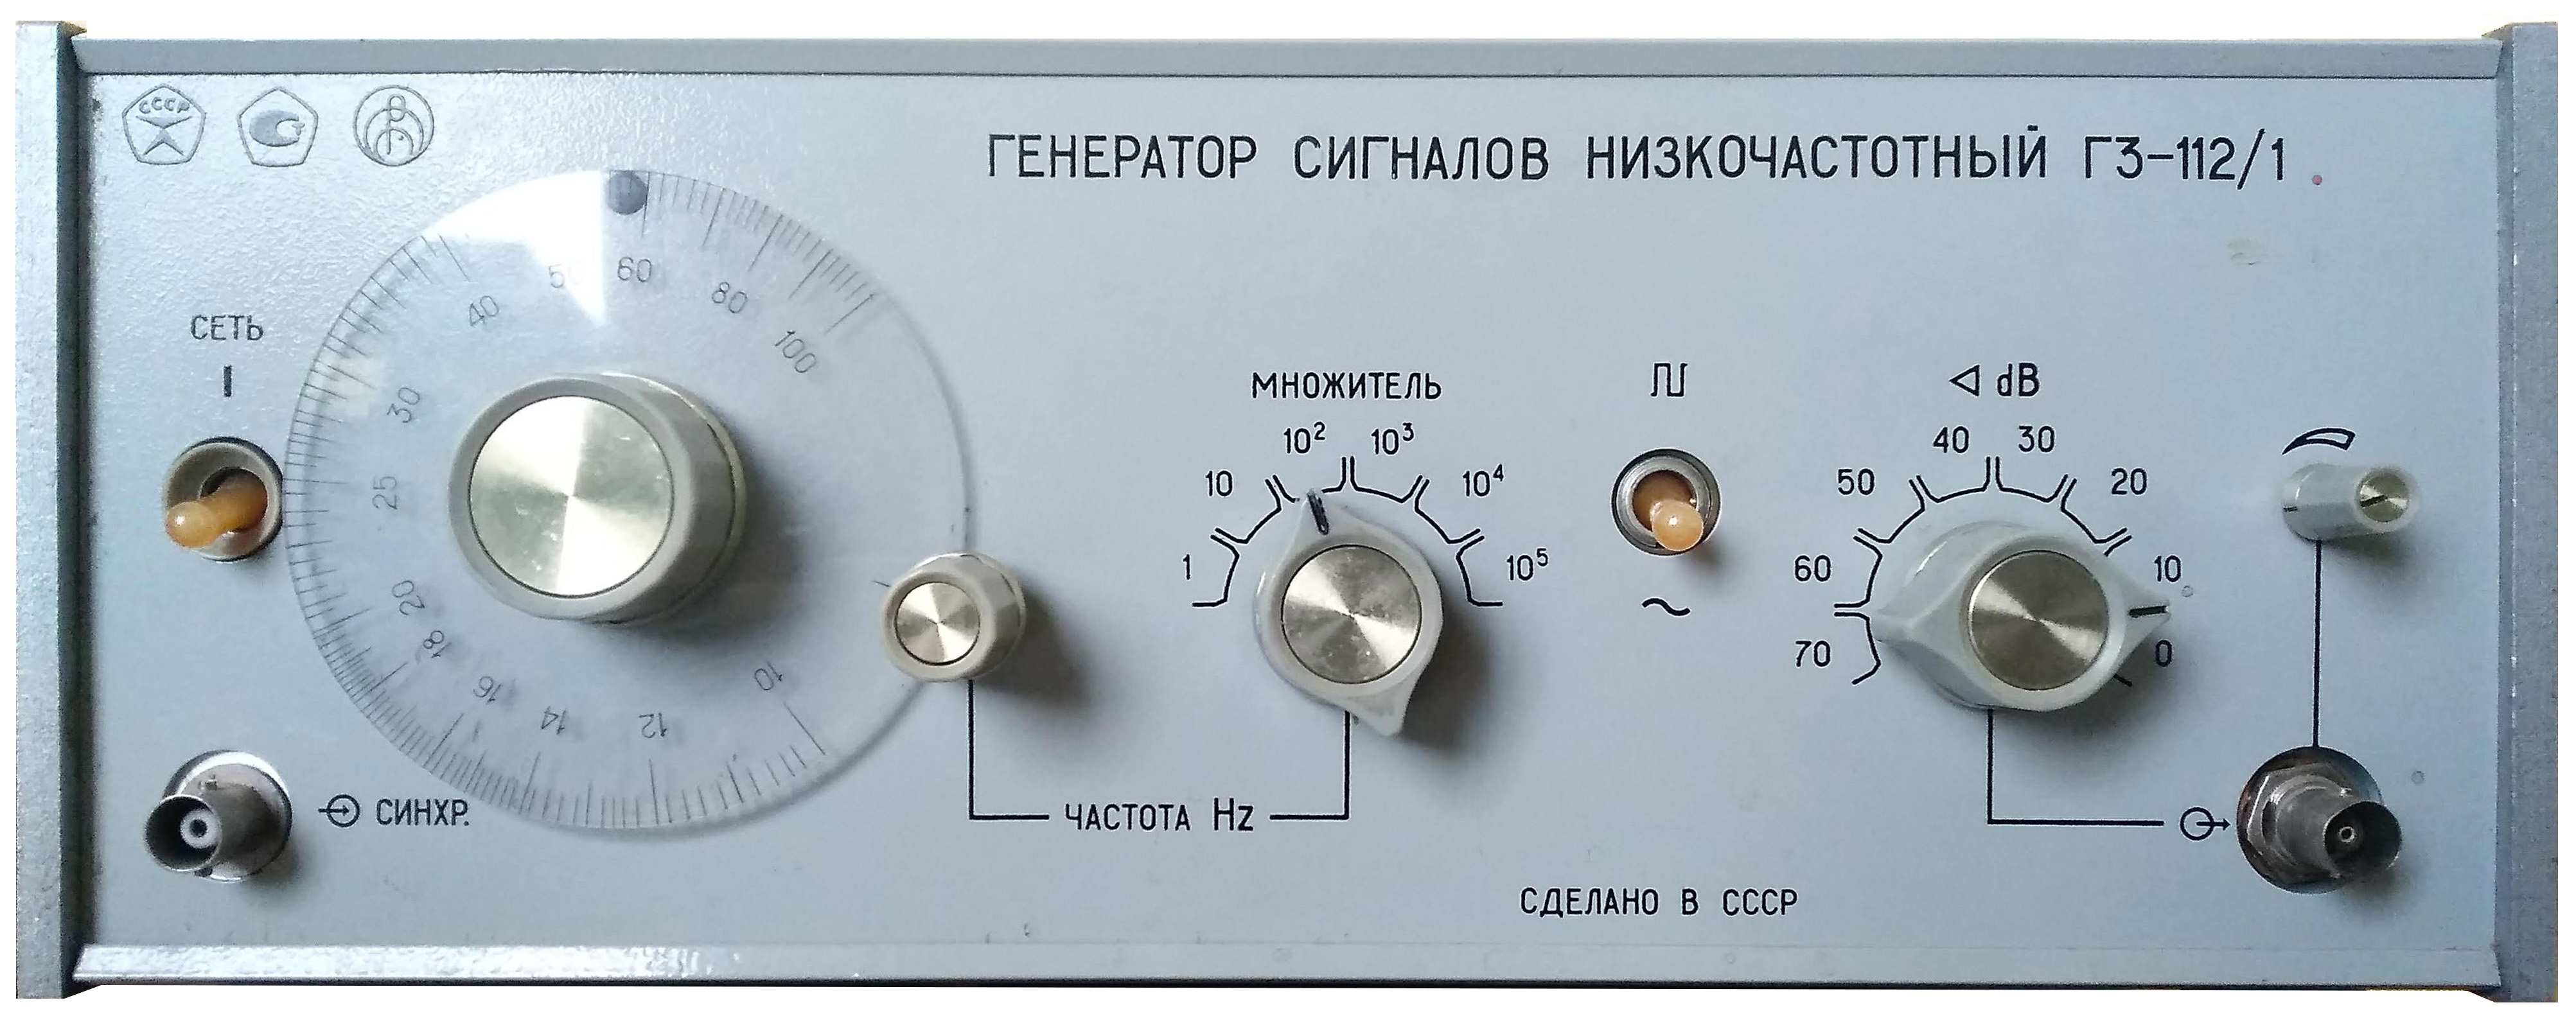
\includegraphics[width=12cm]{\currfiledir/GZ112}};
    \node[small dot,pin={[pin distance=2.2cm]90:{\ref{btn:power}}}] at (-5,0) {};
    \node[small dot,pin={[pin distance=1cm]-90:{\ref{btn:exit}}}] at (5.0,-1.5)  {};
    \node[small dot,pin={[pin distance=1cm]0:{\ref{btn:dB}}}] at (5.1,0.1)  {};
    \node[small dot,pin={[pin distance=2.75 cm]-15:{\ref{btn:dBMultiplier}}}] at (3.5,-0.5)  {};
    \node[small dot,pin={[pin distance=2.3cm]90:{\ref{btn:sygnaltype}}}] at  (1.8,-0.1) {};
    \node[small dot,pin={[pin distance=2.1cm]90:{\ref{btn:Hz}}}] at (-3.3,0.1) {};
    \node[small dot,pin={[pin distance=2.7cm]90:{\ref{btn:HzMultiplier}}}] at (0.3,-0.5) {};
%    \draw[red] (-6,-3) to [grid with coordinates] (6,2.2);
\end{tikzpicture}
\caption{Елементи керування генератором ГЗ-112}
\label{fig:gz112}
\end{figure}

На рис.~\ref{fig:gz112} показані основні органи керування генератором: 
\begin{enumerate}
    \item \label{btn:power} ручка вмикання/вимикання живлення;
    \item \label{btn:Hz} регулювання частоти; 
    \item \label{btn:HzMultiplier} множник частоти вихідного сигналу;
    \item \label{btn:sygnaltype} установка форми сигналу: синусоїдальний/меандр;
    \item \label{btn:dB} регулювання амплітуди вихідного сигналу; 
    \item \label{btn:dBMultiplier} множник амплітуди вихідного сигналу;  
    \item \label{btn:exit} вихід сигналу; 
    \item вивід синхронізації.
\end{enumerate}

\subsubsection*{Диференційний підсилювач}

%---------------------------------------------------------
\begin{wrapfigure}{l}{0.35\linewidth}\centering
    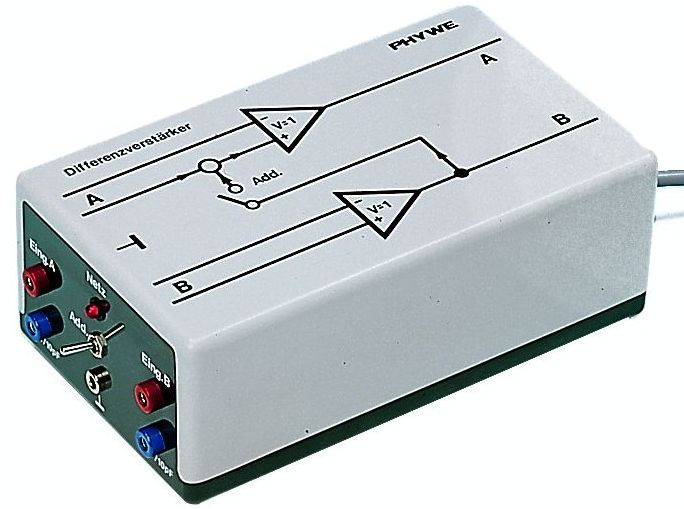
\includegraphics[width=4cm]{\currfiledir/DiffAmpl}
\caption{Диференційний підсилювач}
\label{fig:DiffAmpl}
\end{wrapfigure}%
%---------------------------------------------------------
Диференційний підсилювач (рис.~\ref{fig:DiffAmpl}) призначений для одночасного вимірювання двох напруг при підключенні до входів двоканального осцилографа. Його входи можуть бути підключені до будь-якої точки кола не впливаючи на його електричну поведінку.

Він має два входи, які позначені літерами $A$ та $B$, кожен з яких має пару $4$~мм сокетів червоного та синього кольору. Детальну інформацію можна знайти на сайті \href{https://www.phywe.com/en/difference-amplifier.html#tabs3}{PHYWE}.



\subsubsection*{Осцилограф C1-93}

\begin{figure}[h!]
\centering
\begin{tikzpicture}[every pin/.style={minimum size = 5pt, pin edge={red, thick}, draw, fill=gray!5, red, circle, font=\scriptsize},
    small dot/.style={fill=black,circle,scale=0.3}]

    \node at (0,0){ 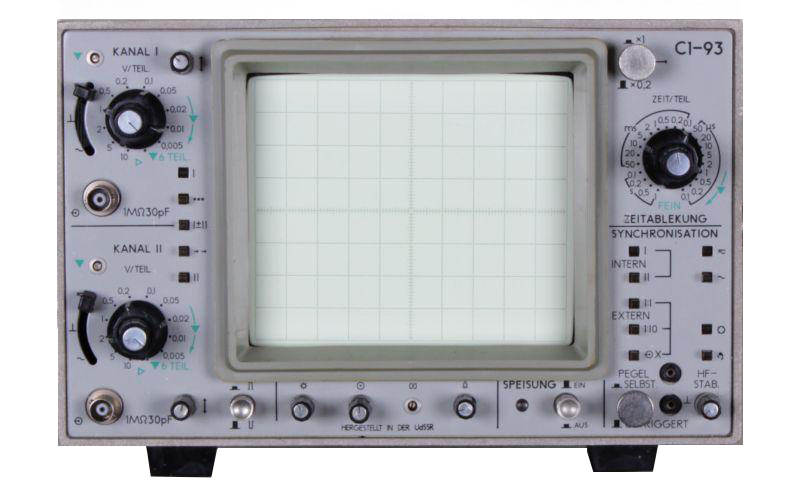
\includegraphics[width=12cm]{\currfiledir/Oscillograph}};
    \node[small dot,pin={[pin distance=1cm]-90:{\ref{btn:power}}}] at (2.6,-2.6)  {};
    \node[small dot,pin={[pin distance=1cm]-90:{\ref{btn:focus}}}] at (-0.6,-2.6)  {};
    \node[small dot,pin={[pin distance=1cm]-90:{\ref{btn:brightness}}}] at  (-1.5,-2.6) {};
    \node[small dot,pin=180:{\ref{btn:gk}}] at (-4.5,0.6) {};
    \node[small dot,pin=160:{\ref{btn:pzch}}] at (-4,1.8) {};
    \node[small dot,pin={[pin distance=1.5cm]120:{\ref{btn:stch}}}] at (-4,2.2) {};
    \node[small dot,pin=90:{\ref{btn:YShift}}] at (-3.3,2.7) {};
    \node[small dot,pin={[pin distance=1cm]-90:{\ref{btn:YShift}}}] at  (-3.3,-2.6) {};
    \node[small dot,pin={180:{\ref{btn:gk}}}] at (-4.5,-2.5) {};
    \node[small dot,pin={[pin distance=1.2cm]180:{\ref{btn:pzch}}}] at (-4,-1.5) {};
    \node[small dot,pin={[pin distance=0.5cm]170:{\ref{btn:stch}}}] at (-4,-1.0) {};
    \node[small dot,pin=0:{\ref{btn:timestepsoft}}] at (4.2,1.2) {};
    \node[small dot,pin={[pin distance=2cm]180:{\ref{btn:ChangeChanels}}}] at (-3.2,-0.2) {};
    \node[small dot,pin={[pin distance=1.5cm]45:{\ref{btn:timestep}}}] at (4.2,1.7) {};
    \node[small dot,pin={[pin distance=1.5cm]-45:{\ref{btn:iternal}}}] at (4.1,-0.4) {};
    \node[small dot,pin={[pin distance=1.5cm]-45:{\ref{btn:external}}}] at (4.1,-1.4) {};
%    \draw[red] (-6,-5) to [grid with coordinates] (6,5);
\end{tikzpicture}

\caption{Елементи керування осциллографом C1-93}
\label{fig:с1-93}
\end{figure}

На рис.~\ref{fig:с1-93} показані основні органи керування осцилографом: 

\begin{enumerate}
    \item \label{btn:power} ручка вмикання/вимикання живлення;
    \item \label{btn:focus}ручка керування фокусуванням електронного променя;
    \item \label{btn:brightness} ручка керування яскравістю  електронного променя;
    \item \label{btn:gk} гніздо <<вхід>> каналів;
    \item \label{btn:pzch} ручка плавної зміни чутливості (в нормі повернута проти годинникової стрілки до упору) каналів;
    \item \label{btn:stch}ручка ступінчатого перемикання чутливості;
    \item \label{btn:YShift}ручка зміщення електронного променя по осі <<Y>> каналів;
%    \item ручка вмикання/вимикання розгортки по осі <<Y>> каналу I;
%    \item \label{btn:gk2} гніздо <<вхід>> канала II;
    \item \label{btn:pzch2} ручка плавної зміни чутливості (в нормі повернута проти годинникової стрілки до упору);
%    \item ручка ступінчатого перемикання чутливості каналу II;
%    \item \label{btn:YShift2}ручка зміщення електронного променя по осі <<Y>> каналу II;
%    \item ручка вмикання/вимикання розгортки по осі <<Y>> каналу II;
    \item \label{btn:ChangeChanels} кнопки перемикання каналів;
    \item \label{btn:timestep}ручка ступінчатої зміни ціни поділок розгортки за часом;
    \item \label{btn:timestepsoft}ручка плавної зміни чутливості розгортки за часом  (в нормі повернута проти годинникової стрілки до упору);
    \item \label{btn:iternal}перемикачі для синхронізації розгортки внутрішнім сигналом;
    \item \label{btn:external}перемикачі для синхронізації розгортки зовнішнім сигналом.
\end{enumerate}

\subsubsection*{Робота осцилографа в режимі внутрішньої розгортки}

При роботі осцилографа в режимі внутрішньої розгортки на канали I та II поступають сигнали, які виводяться на екран у вигляді двох синусоїд (рис.~\ref{fig:InternalMode}).  Зсув фаз між сигналами можна безпосередньо визначити по шкалі на екрані.

\begin{figure}[!h]\centering
    % !TeX program = lualatex
% !TeX encoding = utf8
% !TeX spellcheck = uk_UA
% !TeX root =../LabWork.tex

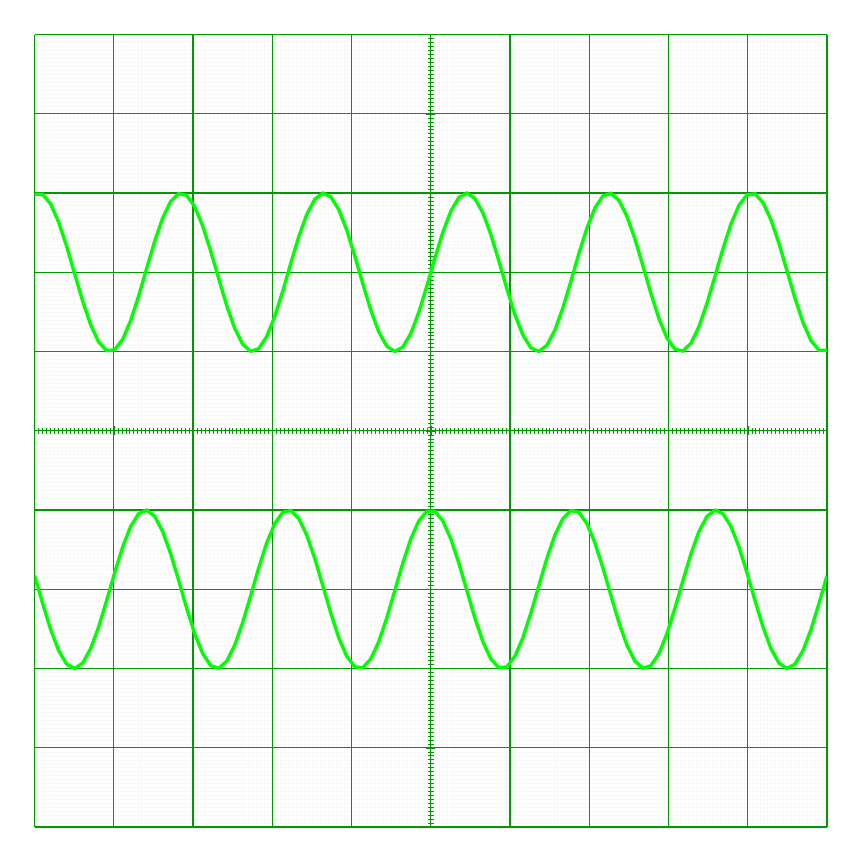
\begin{tikzpicture}[scale=0.75]

\begin{axis}[%
% === Налаштування сітки ===
				grid = both,
				major grid style={line width=.6pt,draw=green!60!black},
				minor tick num = 19,
				minor grid style = {line width=.1pt,draw=gray!5},
				% === Налаштування положення координатних осей ===
				axis lines = middle,
				axis line style={-, green!60!black},
                every x tick/.style={green!60!black},
                every y tick/.style={green!60!black},
width=15cm,
height=15cm,
%scale only axis,
%enlargelimits=false,
%line join=round,
%% === Налаштування сітки ===
				% === Вибір підписів шкали для відображення ===
xticklabel=\empty,
yticklabel=\empty,
extra x ticks={-5,...,5},
extra y ticks={-5,...,5},
xmin = -5,
xmax = 5,
ymin = -5,
ymax = 5,
]

\addplot[samples=100,mark=none, green, ultra thick] {2+sin(200*x)};
\addplot[samples=100,mark=none, green, ultra thick] {-2+sin(200*x+90)};
\end{axis}

\end{tikzpicture}
\caption{Вигляд сигналів на екрані осцилографа, який працює в режимі внутрішньої розгортки}
\label{fig:InternalMode}
\end{figure}


Для переведення в такий режим, необхідно:
\begin{enumerate}
\item  натиснути кнопку  \tcbox{\sc{$\rightarrow\rightarrow$}} перемикання каналів~\circled{\ref{btn:ChangeChanels}};
\item  натиснути перемикач \tcbox{\sc{I}} синхронізації розгортки внутрішнім сигналом~\circled{\ref{btn:iternal}}.
\end{enumerate}


\subsubsection*{Робота осцилографа в режимі осцілоскопу}

При роботі осцилографа в режимі осцилоскопа на канали I та II поступають сигнали, які виводяться на екран у вигляді  \href{https://uk.wikipedia.org/wiki/Фігури\_Ліссажу}{фігури Ліссажу} (рис.~\ref{fig:ExternalMode}). Тип фігури Ліссажу залежить від зсуву фаз між сигналами, що подаються на канали I та II. У випаду, якщо між сигналами зсув фаз дорівнюватиме $\pi/2$ і амплітуди сигналів однакові то на екрані має спостерігатись еліпс (рис.~\ref{fig:ExternalMode}). Якщо ж амплітуди сигналів будуть однакові, то фігура матиме вигляд кола. Майте на увазі, що коректний вигляд фігур можна побачити, якщо ціни поділок  по осям $X$ та $Y$ однакові, для цього ручки \circled{\ref{btn:stch}} повинні мати однакові значення \tcbox{\sc{V/дел}}. Як правило, канал I розгортається по осі $Y$ а канал II по осі $X$.


\begin{figure}[!h]\centering
    % !TeX program = lualatex
% !TeX encoding = utf8
% !TeX spellcheck = uk_UA
% !TeX root =../LabWork.tex

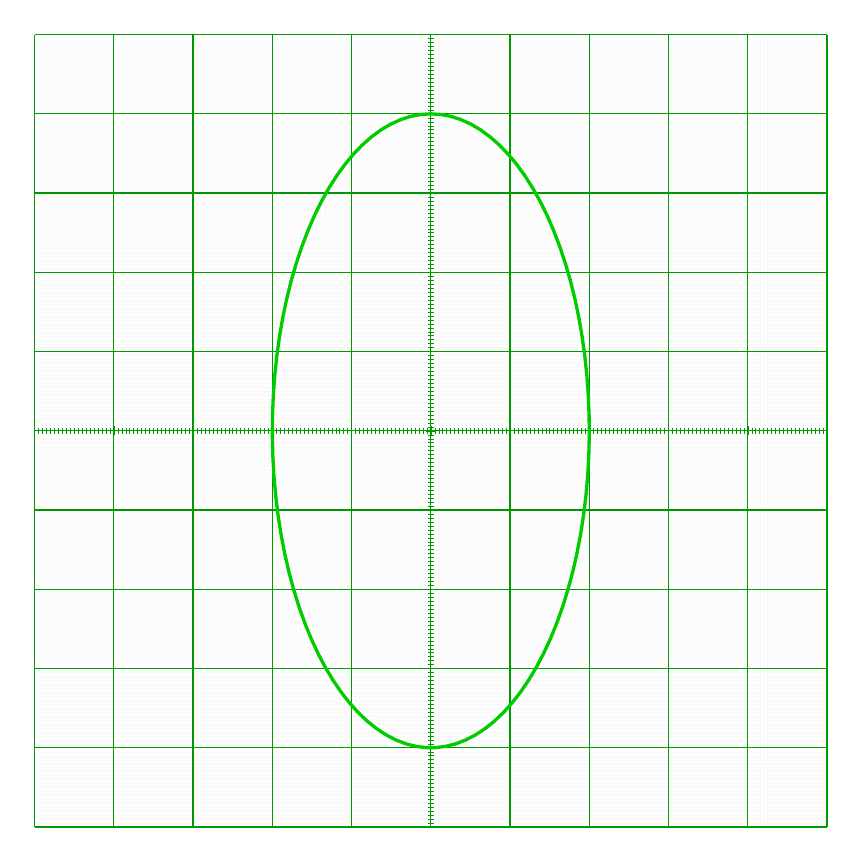
\begin{tikzpicture}[scale=0.75]

\begin{axis}[%
% === Налаштування сітки ===
				grid = both,
				major grid style={line width=.6pt,draw=green!60!black},
				minor tick num = 19,
				minor grid style = {line width=.1pt,draw=gray!5},
				% === Налаштування положення координатних осей ===
				axis lines = middle,
				axis line style={-, green!60!black},
                every x tick/.style={green!60!black},
                every y tick/.style={green!60!black},
width=15cm,
height=15cm,
%scale only axis,
%enlargelimits=false,
%line join=round,
%% === Налаштування сітки ===
				% === Вибір підписів шкали для відображення ===
xticklabel=\empty,
yticklabel=\empty,
extra x ticks={-5,...,5},
extra y ticks={-5,...,5},
xmin = -5,
xmax = 5,
ymin = -5,
ymax = 5,
trig format plots=rad,
]

\addplot[samples=100, mark=none, green!80!black, ultra thick, domain=0:2*pi,] ({2*sin(x)}, {4*cos(x)});
\end{axis}
\end{tikzpicture}%
\caption{Вигляд сигналів на екрані осцилографа, який працює в режимі осцилоскопа}
\label{fig:ExternalMode}
\end{figure}


Для переведення в такий режим, необхідно:
\begin{enumerate}
\item  натиснути кнопку  \tcbox{\sc{II}} перемикання каналів~\ref{btn:ChangeChanels};
\item  натиснути перемикач \tcbox{\sc{\inX}} синхронізації розгортки зовнішнім сигналом~\ref{btn:external}.
\end{enumerate}

\section{Методика дослідження}

\subsection{Опис методики дослідження}

На послідовно з'єднані резистор та конденсатор подають синусоїдальну зовнішню напругу з контрольованою частотою $\omega = 2\pi \nu$, яка задається генератором ГЗ-112. Напруги на конденсаторі і резисторі вимірюються за допомогою  осцилографа C1-93. Знаючи опір резистора можна знайти опір конденсатора, якщо підібрати частоту, на якій напруги, вимірювані осцилографами будуть мати однакову амплітуду.

Для дослідження використовують електричне коло, наведено на рис.~\ref{pic:RC_circuit}.

%=========================================================
\begin{figure}[h!]\centering
        % !TeX program = lualatex
% !TeX encoding = utf8
% !TeX spellcheck = uk_UA
% !TeX root =../LabWork.tex

\begin{tikzpicture}[thick, every circuit symbol/.style={thick}]
	\draw[red, fill=red!10] (-0.5,-1.5) coordinate (G) rectangle ++(1,3);
    \draw[red!50, fill=red!10] (4.7,-1.5) coordinate (Diff)  rectangle ++(1,3);
    \draw[red!50, fill=red!10] (9.5,-1.5) coordinate (Osc)  rectangle ++(1.5,3);
    \node[fill=black,circle,scale=0.3,pin={[pin distance=0.5cm]225:{\scriptsize Генератор ГЗ-112/1}}] at (G) {};
    \node[fill=black,circle,scale=0.3,pin={[pin distance=0.5cm]-45:{\scriptsize Дифференційний підсилювач}}] at (Diff) {};
    \node[fill=black,circle,scale=0.3,pin={[pin distance=0.5cm]-45:{\scriptsize Осцилограф C1-93}}] at (Osc) {};
	\draw (0,-2) coordinate (START) to [ac source={rotate=-90}] ++(0,4) -- ++(3,0) -- ++(0,-0.5) coordinate (R1) to[resistor={info={$R$}}]  ++(0,-1.5) coordinate (C1) to  [capacitor={info={$C$}}] ++(0,-1.5)  coordinate (C2)  -- ++(0,-0.5) -- (START)
	;
    %\draw[dashed] (C1) -- ++(-1,0) to [resistor={info'={$R_C$}, color=red}] ++(0,-1.5) -- (C2);
    \pic (A) at (5,0.75) {amplifier}; 
    \pic (B) at (5,-0.75) {amplifier};
    \draw[red] (R1) -- (A-top) ;
    \draw[] (C1) -- (A-bottom);
    \draw[] (C1) -- (B-top) ;
    \draw[blue] (C2) -- (B-bottom);
    \draw (A-head) -- node[above] {\tiny  \tcbox{\sc{A}} до каналу I осцилографа} ++(4,0) coordinate (O1);
    \draw (B-head) -- node[above] {\tiny \tcbox{\sc{B}}  до каналу II осцилографа}  ++(4,0) coordinate (O2);
    \draw[green!50!black] ([xshift=1ex]O1) sin ++(0.25,0.25) cos ++(0.25,-0.25) sin ++(0.25,-0.25) cos ++(0.25,0.25);
    \draw[green!50!black] ([xshift=1ex]O2) sin ++(0.25,0.25) cos ++(0.25,-0.25) sin ++(0.25,-0.25) cos ++(0.25,0.25);
\end{tikzpicture}
		\caption{Схема дослідження $RC$-кола}
		\label{pic:RC_circuit}
\end{figure}


\section{Хід експерименту}

\subsection*{Вимірювання залежності імпедансу конденсатора від частоти та ємності}
\begin{enumerate}
    \item Виберіть режим внутрішньої розгортки для роботи осцилографа .
    \item Зберіть схему, як показано на рис.~\ref{pic:RC_circuit}. Частоту генератора \tcbox{\sc{ГЗ-112/1}} змінюйте за допомогою ручки~\circled{\ref{btn:Hz}}.
    \item \label{item:X_C} Візьміть конденсатор ємністю $1$~$\mu$Ф. Візьміть резистор з найменшим опором. За допомогою ручки генератора~\circled{\ref{btn:Hz}} підберіть частоту, коли амплітуда напруги на конденсаторі (канал $B$) дорівнюватиме амплітуді напруги на резисторі (канал $A$). Це також означає, що при цій частоті $X_C = R$. Поступово збільшуйте опір резисторів ($10$, $15$, $25$, $50$ $75$, $100$, $150$, $200$~Ом) і знімайте залежність $X_C = f(\nu)$. Перемикніть осцилограф в режим осцилоскопа, переконайтесь, що ви бачите коло на екрані.
    \item  Візьміть конденсатор ємністю $2$~$\mu$Ф. Повторіть вимірювання як зазначено в п.~\ref{item:X_C}.
    \item  З'єднайте конденсатори ємністю $1$~$\mu$Ф та $2$~$\mu$Ф послідовно та повторіть вимірювання вказані в п.~\ref{item:X_C}.
    \item  З'єднайте конденсатори ємністю $1$~$\mu$Ф та $2$~$\mu$Ф паралельно та повторіть вимірювання вказані в п.~\ref{item:X_C}.
    \item \label{item:X_C_plot}За результатами вимірювання побудуйте отримані залежності $X_C = f(\nu)$ в логарифмічних координатах для всіх випадків. Зробіть це на одній координатній площині. Апроксимуйте дані теоретичною залежністю. З параметрів апроксимації визначте ємності конденсаторів та порівняйте їх з номіналом (приклад на рис.~\ref{fig:X_Cnu}). Зробіть висновки.
    \item Зробіть зріз апроксимованих залежностей, побудованих в п.~\ref{item:X_C_plot} для кількох частот і побудуйте залежність імпедансу від ємності $X_C = f(C)$ (приклад на рис.~\ref{fig:X_CC}). Зробіть висновки.
\end{enumerate}

\subsection*{Вимірювання залежності зсуву фаз між струмом в колі та напругою генератора}

\begin{enumerate}[resume]
\item Візьміть конденсатор ємністю $1$~мкФ та резистор опором $100$~Ом. Змінюючи частоту генератора в межах п.~\ref{item:X_C} вимірюйте відношення амплітуди напруги на конденсаторі $U_{0C}$ до амплітуди напруги на резисторі $U_{0R}$. Відношення цих амплітуд є тангенсом зсуву фаз аз між струмом в колі та напругою генератора 
\[
\tg\phi = \frac{U_{0C}}{U_{0R}}.
\] 

Побудуйте залежність зсуву фаз від частоти (приклад на рис.~\ref{fig:tanphi_nu}).
\end{enumerate}

\renewcommand{\floatpagefraction}{.1}
%================================================================================================
\begin{figure}[htbp!]\centering
\begin{subfigure}[t]{0.7\linewidth}\centering
    % !TeX program = lualatex
% !TeX encoding = utf8
% !TeX spellcheck = uk_UA
% !TeX root =../LabWork.tex

\begin{tikzpicture}[trim axis left, trim axis right, declare function={nu=1/(2*pi*100*1e-6);}]
\begin{loglogaxis}[
% === Налаштування сітки ===
grid = both,
grid style={line width=.1pt, draw=gray!10},
major grid style={line width=.2pt,draw=brown!50},
minor grid style = {line width=.1pt,draw=brown!10},
xlabel={$ f $,~Гц},
ylabel={$ X_C $,~Ом},
ylabel style={at={(0.05,1)}, anchor=east, rotate=-90},
width=1\linewidth,
height=1\linewidth,
legend style={font=\scriptsize},
legend pos=north east,
	extra tick style={% changes for all extra ticks
			tick align=outside,
			major grid style={dashed,draw=black}
		},
extra y tick style={
blue,
major tick style={
gray,
},
tick label style={
		yshift=0mm,
/pgf/number format/.cd, fixed, fixed zerofill,
precision=2,
}
},
extra x tick style={
blue,
major tick style={
gray,
},
%			      tick label style={
%					yshift=0mm,
%			        /pgf/number format/.cd, fixed, fixed zerofill,
%			        precision=2,
%			      }
},
	extra x ticks={nu}, 
	extra x tick labels={\pgfmathprintnumberFE[custom exponent=3]{nu}},
    extra y ticks={ 1/(2*pi*nu*3e-6)},
	extra y tick labels={
		\pgfmathprintnumberFE[custom exponent=0]{1/(2*pi*nu*3e-6)},
		}, 
]

\pgfmathsetmacro{\sd}{750}
\pgfmathsetmacro{\fd}{1.6e4}

\pgfplotsinvokeforeach{2/3,1,2,3} {
\addplot[forget plot,thick, domain=\sd:\fd,  smooth, mark=none]
{1/(2*pi*x*#1*1e-6)};
}

\addlegendimage{only marks, mark=square}
\addlegendimage{only marks, mark=*}
\addlegendimage{only marks, mark=o}
\addlegendimage{only marks, mark=triangle}

\legend{{Послідовне з'єднання},$C=1$~мкФ, $C=2$~мкФ, {Паралельне з'єднання}}

\pgfplotsinvokeforeach{15,25,50,75,100,150,200} {
\addplot[domain=\sd:\fd, thick, only marks, mark=square,
nodes near coords={\tiny\pgfmathprintnumberFE[custom exponent=0]{#1}}, every node near coord/.append style={anchor=west}
] coordinates { ({1/(2*pi*#1*(2/3)*1e-6)}, {#1}) };
}

\pgfplotsinvokeforeach{10,15,25,50,75,100,150,200} {
\addplot[domain=\sd:\fd, 
thick, only marks, mark=*,
nodes near coords={\tiny\pgfmathprintnumberFE[custom exponent=0]{#1}}, every node near coord/.append style={anchor=west}
] 
coordinates { ({1/(2*pi*#1*1e-6)}, {#1}) };
}

%\addlegendentry{$C = 1$~мкФ, $C = 2$~мкФ, {паралельне з'єднання}, {послідовне з'єднання}}

\pgfplotsinvokeforeach{10,15,25,50,75,100} {
\addplot[domain=\sd:\fd, 
thick, only marks, mark=o,
nodes near coords={\tiny\pgfmathprintnumberFE[custom exponent=0]{#1}}, every node near coord/.append style={anchor=west}
] coordinates { ({1/(2*pi*#1*2e-6)}, {#1}) };
}


\pgfplotsinvokeforeach{10,15,25,50} {
\addplot[domain=\sd:\fd, thick, only marks, mark=triangle,
nodes near coords={\tiny\pgfmathprintnumberFE[custom exponent=0]{#1}}, every node near coord/.append style={anchor=west}
] coordinates { ({1/(2*pi*#1*3e-6)}, {#1}) };
}


\addlegendimage{only marks,mark=*}
%
%\addplot[thick, domain=\sd:\fd,  smooth, mark=none]
%{1/(x*2E-6)};
%
%%\pgfplotsinvokeforeach{0.1,0.2,...,1} {
%%\addplot[domain=1e5:1e6, thick, smooth, mark=triangle]
%%        coordinates { ({#1*1e6}, {(1/(#1*1e6*2e-6))}) };
%%}
%
%\addplot[thick, domain=\sd:\fd, smooth, mark=none]
%{1/(x*3E-6)};
%
%%\pgfplotsinvokeforeach{0.1,0.2,...,1} {
%%\addplot[domain=1e5:1e6, thick, smooth, mark=square]
%%        coordinates { ({#1*1e6}, {(1/(#1*1e6*3e-6))}) };
%%}
%\addplot[thick, domain=\sd:\fd,  smooth, mark=none]
%{1/(x*(2/3)*1E-6)};

%\pgfplotsinvokeforeach{0.1,0.2,...,1} {
%\addplot[domain=1e5:1e6, thick, smooth, mark=o]
%        coordinates { ({#1*1e6}, {(1/(#1*1e6*(2/3)*1e-6))}) };
%}




\end{loglogaxis}    
\end{tikzpicture}
\caption{$X_C = f(f)$}
\label{fig:X_Cnu}
\end{subfigure}
\\
\begin{subfigure}{0.7\linewidth}\centering
    % !TeX program = lualatex
% !TeX encoding = utf8
% !TeX spellcheck = uk_UA
% !TeX root =../LabWork.tex


\begin{tikzpicture}[trim axis left, trim axis right, declare function={nu=1/(2*pi*100*1e-6);}]
    \begin{axis}[
    % === Налаштування сітки ===
    grid = both,
    grid style={line width=.1pt, draw=gray!10},
    major grid style={line width=.2pt,draw=brown!50},
    minor grid style = {line width=.1pt,draw=brown!10},
    minor tick num=9,
    xlabel={$ C $, Ф},
    ylabel={$ X_C $, Ом},
    ylabel style={at={(0,1)}, anchor=east, rotate=-90},
    width=1\linewidth,
    height=1\linewidth,
    legend style={font=\scriptsize},
    legend entries={,$\nu=\pgfmathprintnumberFE[custom exponent=3]{nu}$  Hz},  
    legend pos=north east,
%    xticklabels={$3$, $2$, $1$, $\frac23$},
%    yticklabels={$1.67$, $2.50$, $5.00$, $7.50$},
    ymin=30,
    ymax=160,
%    ytick={25,45,...,150},
    ]
    

    \addplot[thick, domain=0.6e-6:3e-6, mark=none] {1/(2*pi*nu*x)};

    \pgfplotsinvokeforeach{2/3,1,2,3} {
    \addplot[
    thick, only marks, mark=*,
    nodes near coords={\tiny$\pgfmathprintnumberFE[custom exponent=0]{#1}$}, every node near coord/.append style={anchor=west}
    ] 
    coordinates { (#1*1e-6, {1/(2*pi*nu*#1*1e-6)}) };
    }     
    \end{axis}    
\end{tikzpicture}
\caption{$X_C = f(C)$}
\label{fig:X_CC}
\end{subfigure}
\caption{Залежність імпедансу $X_C$ від частоти $f$ та ємності $C$}
\end{figure}

\begin{figure}[h!]\centering
    % !TeX program = lualatex
% !TeX encoding = utf8
% !TeX spellcheck = uk_UA
% !TeX root =../LabWork.tex

\begin{tikzpicture}[declare function={C=2*10^(-6);R = 100;}]
    \begin{axis}[
    % === Налаштування сітки ===
    grid = both,
    grid style={line width=.1pt, draw=gray!10},
    major grid style={line width=.2pt,draw=brown!50},
    minor grid style = {line width=.1pt,draw=brown!10},
    xlabel={$ f $, Гц},
    ylabel={$\phi$, $\circ$},
    ylabel style={at={(0.1,1)}, anchor=east, rotate=-90},
    axis x line=top,
    every x tick scale label/.style={at={(xticklabel cs:1)},anchor=south west},
    width=0.7\linewidth,
    height=0.7\linewidth,
    legend style={font=\scriptsize},
    legend entries={,{$C = 2$~мкФ {,} $R = 100$~Ом}},  
    legend pos=south east,
    tick label style={scaled x ticks=base 10:-3},
    ]
    \pgfmathsetmacro{\sd}{750}
    \pgfmathsetmacro{\fd}{16e3}

    \addplot[domain=\sd:\fd, thick, samples=100, smooth, mark=none]
    {-atan(1/(2*pi*x*C*R))};


\pgfplotsinvokeforeach{1,2,...,16} {
\addplot[ 
thick, only marks, mark=o,
nodes near coords={\tiny\pgfmathprintnumberFE[custom exponent=0]{#1}}, every node near coord/.append style={anchor=south},
] coordinates { ({#1*1e3}, {-atan(1/(2*pi*#1*1e3*C*R))}) };
}

    
    \end{axis}    
\end{tikzpicture}
    \caption{Залежність зсуву фаз $\phi$ від частоти $f$}
    \label{fig:tanphi_nu}
\end{figure}
%================================================================================================    

\section*{Контрольні запитання}

\begin{enumerate}
	\item Як пояснити, що змінний струм протікає через конденсатор?
	\item Поясніть метод комплексних амплітуд та сформулюйте на їх основі правила Кірхгофа для кіл змінного струму.
	\item Що таке імпеданс?
	\item Що таке активний та реактивний опори?
	\item Побудуйте векторну діаграму паралельного та послідовного $RC$-кола.
	\item Як впливає неідеальність конденсатора на зсув фаз між напругою та струмом на ньому в послідовному та паралельному $RC$-колі?
    \item Як впливає внутрішній опір генератора на результати вимірювань?
    \item Як виміряти зсув фаз за допомогою фігур Ліссажу?
\end{enumerate}

